\documentclass[11pt]{article}
\usepackage{color} %used for font color
\usepackage{amssymb} %maths
\usepackage{amsmath} %maths
\usepackage{bm}
\usepackage{epsfig}
\usepackage{soul}
\usepackage{subcaption}
\usepackage{listings}
\usepackage{authblk}
\usepackage{float}
\usepackage{graphicx}
\usepackage{multicol}
\usepackage{lipsum}
\topmargin-.5in
\textwidth6.6in
\textheight9in
\setlength{\columnsep}{0.6cm}
\oddsidemargin0in
\setlength\parindent{0pt}

%\def\fs{\scriptsize}
\usepackage{listings}
\usepackage{xcolor}

\DeclareMathOperator*{\E}{\mathbb{E}}

%New colors defined below
\definecolor{codegreen}{rgb}{0,0.6,0}
\definecolor{codegray}{rgb}{0.5,0.5,0.5}
\definecolor{codepurple}{rgb}{0.58,0,0.82}
\definecolor{backcolour}{rgb}{0.95,0.95,0.92}

%Code listing style named "mystyle"
\lstdefinestyle{mystyle}{
  backgroundcolor=\color{backcolour},   commentstyle=\color{codegreen},
  keywordstyle=\color{magenta},
  numberstyle=\tiny\color{codegray},
  stringstyle=\color{codepurple},
  basicstyle=\ttfamily\footnotesize,
  breakatwhitespace=false,         
  breaklines=true,                 
  captionpos=b,                    
  keepspaces=true,                 
  numbers=left,                    
  numbersep=5pt,                  
  showspaces=false,                
  showstringspaces=false,
  showtabs=false,                  
  tabsize=2
}

%"mystyle" code listing set
\lstset{style=mystyle}

\title{ \bf{Assignment III \\ MA797: Special Topics in Machine Learning}}
\author{Alp Tezbasaran$^{a}$}
\affil{\textit{$^{a}$Department of Nuclear Engineering NCSU, alptezbasaran@ncsu.edu}}
\date{October 25, 2019}
\begin{document}
\maketitle

\section{Artificial Neural Network}

In the second assignment, a perceptron classifier is written and used to classify high dimensional data with given hyper-parameters. The task here is to use the same data, and investigate if a higher accuracy values can be achieved when feed-forward artificial neural network is used as a classifier. For this task, Tensorflow2 is used to construct multi-layer perceptron with requested structure.

\begin{lstlisting}[language=Python, basicstyle=\tiny, caption=Python code for ANN]
tf.__version__
tf.random.set_seed(0)

tf.keras.backend.clear_session
# A3 Q1 data

data = sio.loadmat('SampleCredit.mat')
X_train = data['sample'][0:500,]
X_test  = data['sample'][500:,]
y_train = data['label'][0:500,0].reshape(500,1)
y_test  = data['label'][500:,0].reshape(X_test.shape[0],1)

y_train[y_train==-1] = 0
y_test[y_test==-1] = 0


# Normalization
for i in range(X_train.shape[1]):
  X_train[:,i] = np.divide(X_train[:,i],max(X_train[:,i]))
  X_test[:,i] = np.divide(X_test[:,i],max(X_test[:,i]))

#Keras sequential
model = tf.keras.models.Sequential()
# The first layer
model.add(tf.keras.layers.Dense(units = 30, activation = 'linear', input_shape = (15, )))
#model.add(tf.keras.layers.Dropout(0.5))
model.add(tf.keras.layers.Dense(units = 30, activation = 'tanh'))
#model.add(tf.keras.layers.Dropout(0.5))
model.add(tf.keras.layers.Dense(units =  2, activation = 'softmax'))
# Compiling
model.compile(optimizer='adam' ,loss='sparse_categorical_crossentropy', metrics=['accuracy'])
# Summary
model.summary()

# Tensorboard
log_dir = 'log'+ datetime.datetime.now().strftime("%Y%m%d-%H%M%S")
tensorboard_callback = tf.keras.callbacks.TensorBoard(log_dir=log_dir, histogram_freq=1)

# Fit
model.fit(X_train, y_train, use_multiprocessing = True , validation_data = (X_test, y_test) ,epochs = 1000, callbacks=[tensorboard_callback])
# Eval
test_loss, test_accuracy = model.evaluate(X_test,y_test, verbose = 0)
test_loss, test_accuracy
\end{lstlisting}

The code has a few sections. First one is the importing of required libraries. The 'numpy' is used to arrange data types and basic mathematical operations, 'sio' is to import 'Excel' data into python, and finally 'tensorflow' is used for to train an artifical neural network. \medskip

Second section is the data import part. As specified in the assignment, first 500 data points are used for training and the rest is for testing. \medskip

Normalization part divides each feature points with the maximum value of the corresponding feature. This part is used only in the second part of the question. \medskip

The remaining part is the Tensorflow implementation of specified network structure. Here first the \underline{model} object is created from \emph{Sequential} class of \emph{tensorflow.keras} module. \emph{Sequential} class is used to construct feed-forward networks, where outputs of each layer is sent to the following one. This class also allows users to specify different layers (Dense, Conv, etc.), and has a compilation method with different optimizers (SGD, Adam, RMDprop, etc.), various metrics (accuracy, crossentropy, cosine proximity, etc.), and losses (mean squared error, mean absolute error, hinge, logcosh, etc.). \medskip

The model is compiled with \emph{adam} optimizer to minimize the loss of \emph{sparse categorical cross entropy}. This loss is used to calculate categorical entropy when labels don't have one-hot encoded structure. The metric to optimize is the \emph{accuracy} which is the fraction of correct predictions. \medskip

The \emph{fit} method is where the model is trained, here \emph{epocs} is picked as 1000 because the previous assignment had value for epocs 1000. \medskip

Testing data accuracy is evaluated with \emph{evaluate} method of the \emph{Sequantial} class. This method basically predicts the classes for all the testing data and calculates the fraction of correctly predicted data. The following figure shows the accuracy evaluation. \medskip

The network structure is specified in the assignment.
\begin{itemize}
    \item First layer: 30 neurons - linear transfer function
    \item Second layer: 30 neurons - hyperbolic tangent activation function
    \item Third (output) layer: 2 neurons -  softmax activation fuction
\end{itemize}

\bgroup
\def\arraystretch{1.5}%  1 is the default, change whatever you need
\begin{table}[H]
\centering
\caption{Testing accuracy of ANN and perceptron(no-tune)}
\begin{tabular}{|c|c|c|}
\hline
Data        &  ANN      & Perceptron \\ \hline
(a) Raw         &  0.732    & 0.680  \\ \hline
(b) Normalized  &  0.791    & 0.622  \\ \hline
\end{tabular}
\label{table:q1acc}
\end{table}
\egroup

Table \ref{table:q1acc} shows test accuracy values for both ANN and perceptron (Assignment 2 Question 2) models. It is noteworthy that the perceptron model, is the un-tuned one, meaning the model trained with the given hyperparameters.\medskip

Figures suggest that the testing accuracy is much better than that of perceptron. This means that the ANN model performs much better than a mere perceptron. 

\newpage
\section{Linear Classifiers}

Following points in two different classes are to be used to train linear classifiers.

\begin{align*}
    &C_1 (1):  \quad (1, 3)^T \ (2, 3)^T \ (2, 4)T  \\
    &C_2 (-1): \quad (3, 1)^T \ (3, 2)^T \ (4, 2)^T
\end{align*}

\subsection*{(a) Support Vector Machines} 
\subsubsection*{(i)}

Given data is shown in Figure \ref{fig:data}
\begin{figure}[H]
\centering
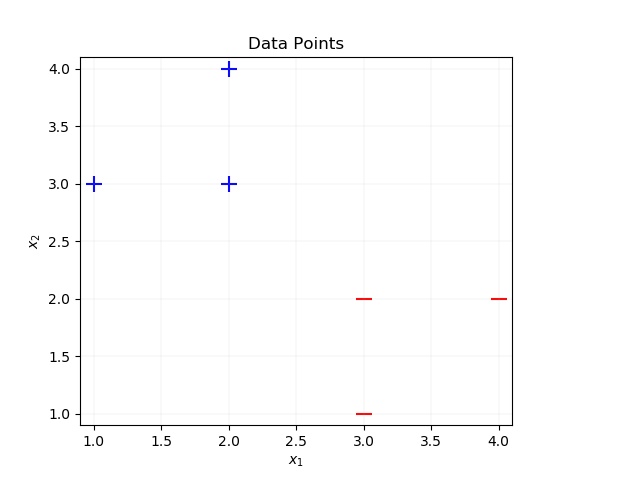
\includegraphics[width=0.65\columnwidth]{pics/data.png}
\captionsetup{justification=centering}
\caption{Data Points and Labels}
\label{fig:data}
\end{figure}

Intuitively one can say that this data is linearly separable and the optimal hyperplane that separates classes, is 
\begin{equation*}
    x_2 = x_1
\end{equation*}
which makes $\bm{w}$ and $b$,
\begin{align*}
    &\bm{w} = [-1 \quad 1] \\
    &b = 0
\end{align*}

The support vectors are the data that has different labels where the margin between the classes is maximized. The closest (minimum euclidean distance) data points that have different labels are;

\begin{align*}
    SV_1 : (2,3)^T \\
    SV_2 : (3,2)^T
\end{align*}

There are only two Support Vectors for this data set.

\subsubsection*{(ii)}

Solution will be made on the dual formulation. \medskip

After defining Lagrangian multiplier and dual formulation following expression is derived.
\begin{equation*}
    h(\lambda) = \sum_{i=1}^N \lambda_i - \frac{1}{2} \sum_{i=1}^N \sum_{j=1}^N y_i y_j \lambda_i \lambda_j \bm{X}^T(i) \bm{X}(j)
\end{equation*}

This is the quadratic objective function expression to maximized for $\lambda$. A general form of the quadratic programming problem can be written as;
\begin{align*}
    \max_{\lambda \geq 0} \quad  &\bm{\lambda}^T \bm{1}- \frac{1}{2} \bm{\lambda}^T Q \bm{\lambda} \\ 
    s.t.     \quad               &\bm{\lambda} \geq \bm{0} \\
                                &\bm{\lambda}^T\bm{y} = 0
\end{align*}

Since the problem definition asks to define the dual problem, solution of this problem is calculated via external quadratic programming solver. All the relative matrices are defined as arguments for solver, and optimum solution for $\lambda$ is returned based on the arguments. After that using KKT conditions, hyperplane weights and bias are calculated.

\begin{align*}
    \bm{w} = \sum_{i = 1}^ N = \bm{\lambda ^ *}_i \bm{X}(i)
\end{align*}

\begin{align*}
    b^* = \frac{1-y_i \bm{w}\bm{X}(i)}{y_i}
\end{align*}

For the quadratic programming problem the solver, \emph{CVXOPT} is used. This is a python package created to solve convex optimization problems, takes arguments of SVM problem as an input and returns $\bm{\lambda}$ values for the dual problem. The definitions of each matrix is as follows.

\begin{align*}
    \bm{\lambda} = 
    \begin{bmatrix}
        \begin{array}{c}
            \lambda_1 \\
            \lambda_2 \\
            \vdots \\
            \lambda_N
        \end{array}   
    \end{bmatrix}_{n\times 1}
    \bm{1} = 
    \begin{bmatrix}
        \begin{array}{c}
            1 \\
            1 \\
            \vdots \\
            1
        \end{array}   
    \end{bmatrix}_{n\times 1}
    \bm{y} = 
    \begin{bmatrix}
        \begin{array}{c}
            y_1 \\
            y_2 \\
            \vdots \\
            y_N
        \end{array}   
    \end{bmatrix}_{n\times 1}
\end{align*}


\begin{align*}
    Q = 
    \begin{bmatrix}
        \begin{array}{cccc}
            y_1y_1\bm{X}_1^T\bm{X}_1 & y_1y_2\bm{X}_1^T\bm{X}_2 & \cdots  &y_1y_N\bm{X}_1^T\bm{X}_N \\
            y_1y_2\bm{X}_1^T\bm{X}_1 & y_1y_2\bm{X}_1^T\bm{X}_1 & \cdots & y_2y_N\bm{X}_2^T\bm{X}_N \\
            \vdots & \vdots & & \vdots \\
            y_Ny_2\bm{X}_N^T\bm{X}_1 & y_Ny_2\bm{X}_N^T\bm{X}_1 & \cdots & y_Ny_N\bm{X}_N^T\bm{X}_N
        \end{array}   
    \end{bmatrix}_{n\times n}
\end{align*}

\newpage
The $\bm{Q}$ matrix calculated from data is;
\begin{align*}
    Q = 
    \begin{bmatrix}
        \begin{array}{rrrrrr}
            10.&  11.&  14.&  -6.&  -9.& -10.\\
             11.&  13.&  16.&  -9.& -12.& -14.\\
             14.&  16.&  20.& -10.& -14.& -16.\\
             -6.&  -9.& -10.&  10.&  11.&  14.\\
             -9.& -12.& -14.&  11.&  13.&  16.\\
            -10.& -14.& -16.&  14.&  16.&  20.
        \end{array}   
    \end{bmatrix}_{n\times n}
\end{align*}

After calculating $\bm{Q}$ and defining, vectors for $\bm{\lambda}$, $\bm{y}$, and $\bm{y}$, all these matrices are converted into \emph{cvxopt} matrix format and used as input for the solver. The solver calculated the following $\lambda$ values.

\begin{align*}
    \bm{\lambda} = 
    \begin{bmatrix}
        \begin{array}{c}
            7.8e-13\\
            1   \\
            7.8e-13 \\
            7.8e-13 \\
            1 \\
            7.8e-13
        \end{array}   
    \end{bmatrix}_{n\times 1}
\end{align*}

After calculating the $\bm{\lambda}$ vector, weights $w$ and the bias $b$ is calculated with the expressions shown above.

\begin{align*}
    &\bm{w} = [-1 \quad 1] \\
    &b = 2\times 10^{-13}
\end{align*}

The bias is basically a small number assigned for numerical stability and can be considered as 0. Figure \ref{fig:hyper} shows the plot for this solution. The hyperplane and support vectors are shown. There are 2 support vectors. This optimal solution matches with the line intuitively predicted hyperplane as well as LDA solution(next section).    

\begin{figure}[H]
\centering
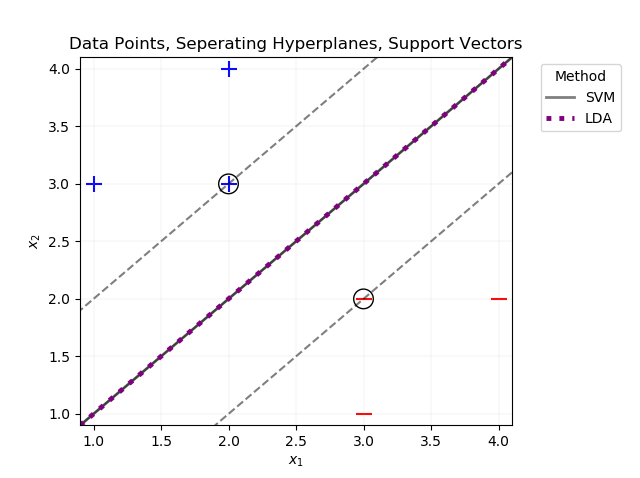
\includegraphics[width=0.65\columnwidth]{pics/hyperplanes.png}
\captionsetup{justification=centering}
\caption{Calculated hyperplanes with SVM and LDA (overlapping), support vectors, data points and labels}
\label{fig:hyper}
\end{figure}

The code for calculations is;

\begin{lstlisting}[language=Python, basicstyle=\tiny, caption=SVM Implementation]
# Importing the libraries
import numpy as np
import matplotlib.pyplot as plt

#Importing with custom names to avoid issues with numpy / sympy matrix
from cvxopt import matrix as cvxopt_matrix
from cvxopt import solvers as cvxopt_solvers


# Data
X = np.array([
  [1., 3.],
  [2., 3.],
  [2., 4.],
  [3., 1.],
  [3., 2.],
  [4., 2.],
])

y = np.array([1,1,1,-1,-1,-1])

#Initializing values and computing H. Note the 1. to force to float type
m,n = X.shape
y = y.reshape(-1,1) * 1.
X_dash = y * X
H = np.dot(X_dash , X_dash.T) * 1.      # Q, done

#Converting into cvxopt format
P = cvxopt_matrix(H)                    # Q, done
q = cvxopt_matrix(-np.ones((m, 1)))
G = cvxopt_matrix(-np.eye(m))
h = cvxopt_matrix(np.zeros(m))
A = cvxopt_matrix(y.reshape(1, -1))
b = cvxopt_matrix(np.zeros(1))

#Setting solver parameters (change default to decrease tolerance)
cvxopt_solvers.options['show_progress'] = True
cvxopt_solvers.options['abstol'] = 1e-10
cvxopt_solvers.options['reltol'] = 1e-10
cvxopt_solvers.options['feastol'] = 1e-10

#Run solver
sol = cvxopt_solvers.qp(P, q, G, h, A, b)
lambdas = np.array(sol['x'])

#w parameter in vectorized form
w = ((y * alphas).T @ X).reshape(-1,1)

#Selecting the set of indices S corresponding to non zero parameters
S = (lambdas > 1e-4).flatten()

#Computing b
b = y[S] - np.dot(X[S], w)

#Display results
print('Ayak = ',lambdas[lambdas > 1e-4])
print('w = ', w.flatten())
print('b = ', b[0])
\end{lstlisting}

\subsection{(b) Linear Discriminant Analysis}
The final linear classifier used is Linear Discriminant Analysis (LDA) method to find a separating hyper-plane between classes. \medskip

LDA classifier, is an optimal classifier where the hyper-plane is calculated analytically. The insight behind this classifier is the projection of data points into new axes where originally inseparable data becomes separable. The new plane maximizes the distance between means of each class and minimize the variance of classes. \medskip

Fisher's optimality criterita is;
\begin{equation*}
    \bm{w^*}= arg\max_{w} \frac{\bm{w^T\mu_1-w^T\mu_{-1}}}{n_1\bm{w^T\Sigma_1}+n_2\bm{w^T\Sigma_{-1}}}
\end{equation*}
where $\bm{w}$ is the hyper-plane, $\bm{\mu}$ is the mean of a class, and $\bm{\Sigma}$ is the covariance matrix calculated for each class separately. \medskip

After algebraic manipulations, an analytical expression is achieved. The optimal hyper-plane is calculated with the following expression.
\begin{equation*}
    \bm{w^*} = (n_1\bm{\Sigma_1}+n_2\bm{\Sigma_{-1}})^{-1}(\bm{\mu_1}-\bm{\mu_{-1}})
\end{equation*}

And predictions (C for class) are made;
\begin{equation*}
    C=sign(w_0+\bm{w^TX})
\end{equation*}

Here, $w_0$ is unknown, but can easily be calculated from the labels.

\begin{align*}
    w_0 &= \E[y_i - \bm{w^{*^T}X}(i)]  \\
        &\frac{1}{N}\sum_i^N (y_i - \bm{w^{*^T}X}(i))
\end{align*}

The above expressions are implemented with \emph{python}.
\begin{lstlisting}[language=Python, basicstyle=\tiny, caption=LDA Implementation]
# Data
X = np.array([
  [1., 3.],
  [2., 3.],
  [2., 4.],
  [3., 1.],
  [3., 2.],
  [4., 2.],
])

y = np.array([1,1,1,-1,-1,-1])


n1 = len(X[ y ==  1])         # Number of points label ' 1'
n2 = len(X[ y == -1])         # Number of points label '-1'

# LDA Implementation
np.set_printoptions(2)

# Calculate Means of Each Feature [2 x 2] 2 classes, 2 features
m1 = np.mean(X[y == 1], axis = 0)
m2 = np.mean(X[y == -1], axis = 0)

m1
m2

# Calculate the Covariance Matrices [2, 2]
var1 = 1/(n1 - 1) * np.dot((X[ y ==  1] - m1).T,(X[ y ==  1] - m1))     # (X[ y ==  1] - m1).shape = [3x2] 3 points, 2 features
var2 = 1/(n2 - 1) * np.dot((X[ y == -1] - m2).T,(X[ y == -1] - m2))     # (X[ y == -1] - m1).shape = [3x2] 3 points, 2 features

# Shared Covariance Matrix
S = n1 * var1 + n2 * var2
S
# Estimate the weights
w_new = np.dot(np.linalg.inv(S), m1-m2)

w0_new = np.zeros(1)
for i in range(X.shape[0]):
  w0_new += y[i]-np.dot(w_new.T,X[i,:])

w0_new = w0_new/X.shape[0]
\end{lstlisting}

Calculated hyperplane for this data;
\begin{align*}
    &\bm{w} = [-1 \quad 1] \\
    &b = 0
\end{align*}
    
The lines up to 11 are the data definition. Then the following lines are used to define mean and variance parameters. Line 35 is where the new weights are calculated and the following loop is where $w_0$ is computed. \medskip

The separating hyperplane calculated with SVM and LDA is the \textbf{\underline{same}} for this data. This means that the assumptions made when deriving LDA solution hold perfectly. The hyperplanes will be the same, if and only if the covariance of classes are the same.

\end{document}
